
\paragraph{Collection Procedure}
\label{sect:mn_verification}

We recruited annotators from Amazon Mechanical Turk\footnote{
	\url{https://mturk.com}
} (AMT) to categorize the object-name pairs from \mn.
Since this is a multiple-choice task we were able to conduct rigorous quality control, ensuring the reliability of these annotations (see the supplementary material for details).
We ran all the \mn data (response sets) through our verification, with two exceptions: 
response sets with $100$\%~agreement (i.e.,~all annotators gave the same name for an object) are treated as correct, and all names with a count of~$1$ considered unreliable.
The remaining $19,427$~objects (on average $4$ names each), were presented to $3$~annotators each (i.e., an image with the object highlighted by its bounding box), with a list of all its names to be verified (see Figure~1 in the supplementary material).
They were asked to judge the ``adequacy''\footnote{
	In the task we provided the definition that \textit{a name is ``adequate'' if there is an object in the image, whose visible parts are tightly circumscribed by the red bounding box, that one could reasonably call by that name}.
} of each name on a 3-point scale: ``perfectly adequate'', ``there may be a (slight) inadequacy'' and ``totally inadequate'' (we will encode these below as 1.0, 0.5 and 0.0, respectively).
If they did not select ``adequate'' they had to specify the type of inadequacy, choosing between ``linguistic mistake'', ``named object not tightly in bounding box",  ``named object mistaken for something it's not'', and ``something else''.
Lastly, annotators were asked to judge which names were likely intended for the same object, through an interface where they would assign the same color to names for the same object.
%% SHORTENING %% Note that this is independent of name adequacy: ``cow'' can be adequate and ``horse'' inadequate, yet both could be intended as naming the same object (i.e., a cow that one annotator misinterpreted to be a horse).
Overall, $255$~participants annotated a total of $69,356$~object-name pairs, with three participants per pair.

%\mw{I think the following is nice, but strictly redundant, so candidate for deletion if need be:}
%Summing up, we provide new verification of \mn, in the form of: name adequacy judgments, type of inadequacy (linguistic, bounding box, named object misinterpreted, other), and information about which names were likely intended for the same object. In relation to our research goal, in section~\ref{sec:analysis} these results will allow us to quantify, for instance, whether the name generated by a given model, if it is not the entry-level name, is at least a name that could reasonably be for the same object as the entry-level name, and whether it is adequate.



%We implemented this verification task on Amazon Mechanical Turk (\url{https://mturk.com}). 

\paragraph{Judgment Aggregation}
We aggregate our name adequacy judgments by taking the mean, and inadequacy type judgments by taking the majority.
%% SHORTENING %%  (counting ``none'' for annotators saying there is no inadequacy). 
Average name adequacy, on the scale from totally inadequate (0) to adequate (1), is 0.80 (\mbox{std=$0.093$}).
The proportion of annotators agreeing on adequacy ratings is 88\%, agreeing on inadequacy type is 86\%, and agreeing on whether two names were intended for the same object is 94\%.
This is high given the complexity of the task
%% SHORTENING %% , essentially mind-reading what the original \mn annotators may have meant, 
and the fact that pictures and bounding boxes are sometimes unclear.
Figure~\ref{fig:verification-piechart} shows the proportion of adequate names and inadequacy types.
\begin{figure}[t]
	\centering
	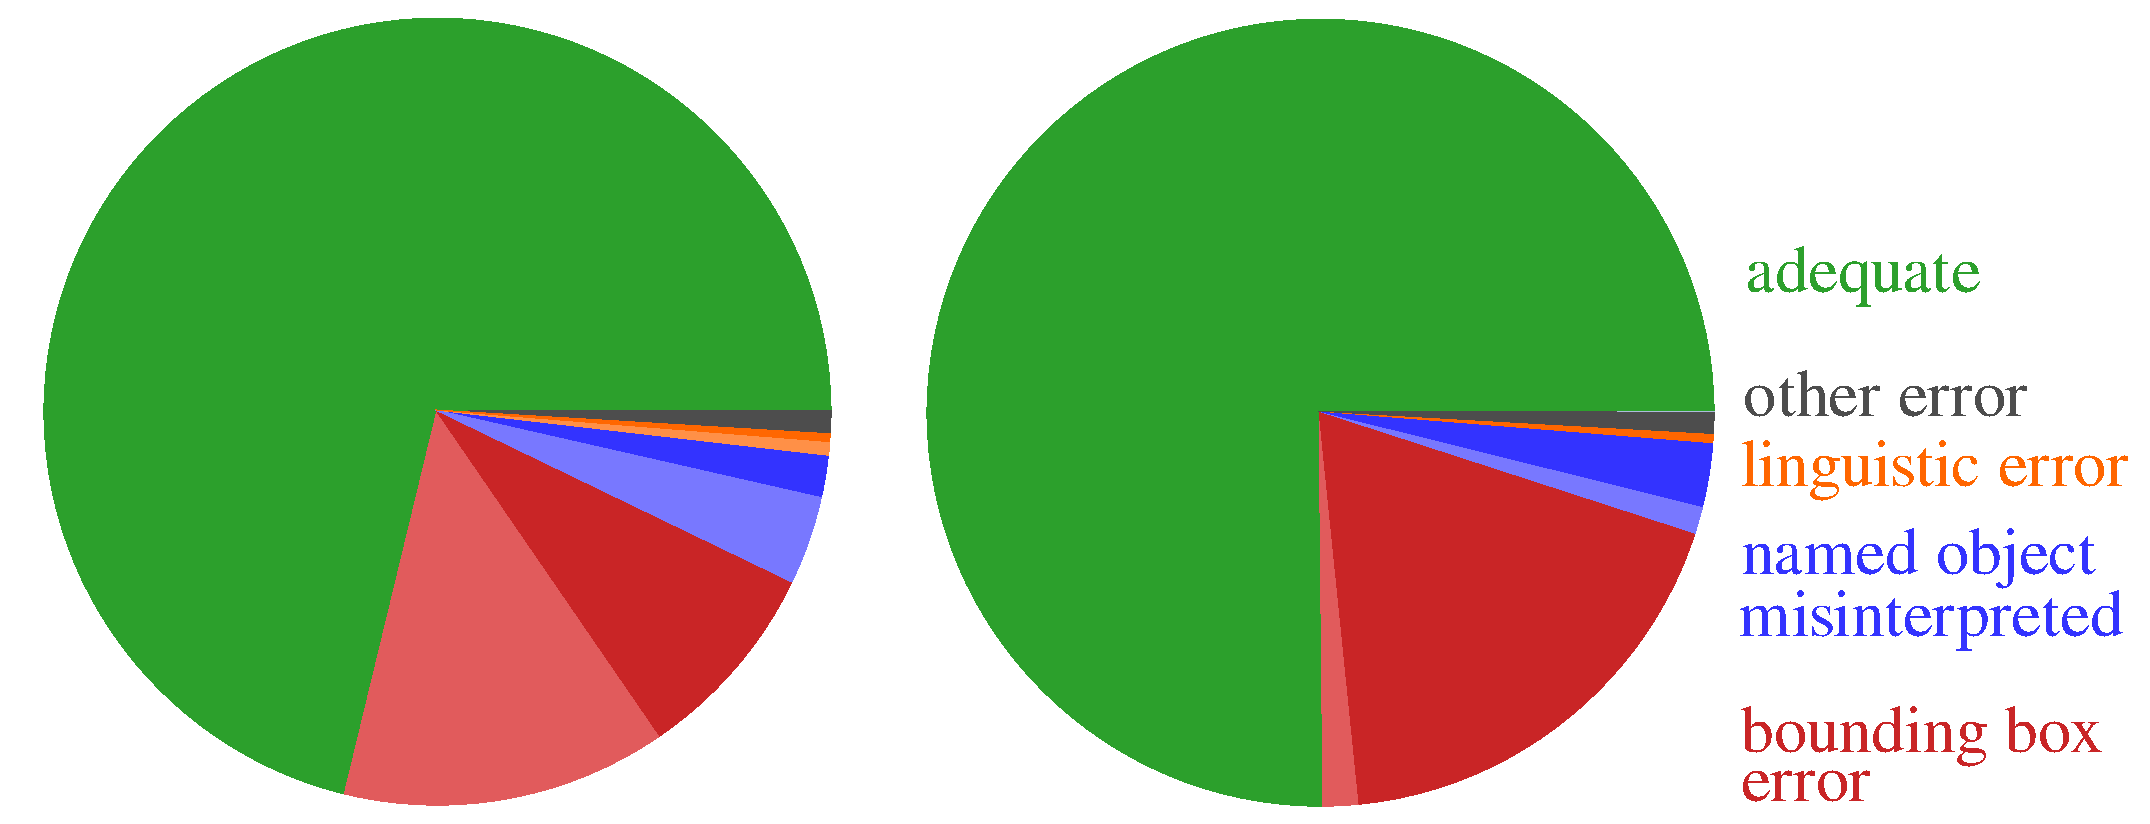
\includegraphics[width=\columnwidth]{images/verification_piechart_double.pdf}\\
	\hspace*{\fill}a.\hspace*{\fill}\hspace*{\fill}b.\hspace*{\fill}\hspace*{\fill}
	\caption{Verification results: a. counting individual annotations; b. counting image-name pairs with their aggregated scores. Lighter shade within a hue indicates slight/possible error of that type; darker shade severe error.}
	\label{fig:verification-piechart}
\end{figure}

We aggregate the judgments of whether two names were intended for the same object in two ways, for different purposes: \sameobject and \cluster.
% \cs{This pair-wise view is only because of the need for aggregating the clustering of 3 annotators into one, isn't it? In this case, it would be "aggregating name cluster", no?! So what you did for the first aggregation (modeling) was a pair-wise aggregation?} \mw{I don't understand this...}
First, for analysing computational object naming models (Section~\ref{sec:analysis}), 
% we want to have all valid name alternatives to the entry-level name (or a target name in general), i.e.,~a soft clustering of names. 	% <- Carina's reformulation, but not strictly true and not clear to me.
we want to know primarily whether the name predicted by a model, if it isn't the entry-level name, was at least intended for the same object as the entry-level name.
This \textbf{\sameobject} measure we compute by a simple majority rule: true if name1 and name2 were judged to be for the same object by a majority of annotators, and false otherwise.
Second, for a better understanding of the verified \mn data itself (analysis below) we want to be able, e.g., to assess the mean number of names per object, and for that we need to compute actual \emph{clusters} of names (the pairwise majority rule does not result in a proper clustering). 
We compute the \textbf{\cluster} of a name by agglomerative, complete-linkage clustering with a distance threshold of .5, using as distance between two names the proportion of annotators saying they do not name the same object (i.e., this means that all pairs of names in a cluster must name the same object according to a majority of annotators).\footnote{
	The `hard' clustering we use may occasionally lead us to \emph{under}estimate the number of names for an object (this is also why we will use \sameobject and not \cluster in model analysis). The alternative, \emph{soft} clustering (where each name could potentially be in multiple clusters), would risk \emph{over}estimating the number of names per object, as well as the number of named objects in an image.
}


%A possible disadvantage of this (hard) clustering method is that every name can only be in one cluster, i.e., name only one object.
%It entails for instance that \emph{food} cannot be clustered both with \emph{pizza} and with the \emph{cheese} on top, even though both are definitely instances of food.
%But this is not as problematic as it may seem, because we do not care primarily about such taxonomic relationships--- %(which could be gotten from, e.g., WordNet) -- 
%rather, we care about which single object a person who entered \emph{food} was likely intending to name: presumably the pizza as a whole rather than the cheese on top. 
%Moreover, although hard clustering may occasionally lead us to \emph{under}estimate the number of names for an object, the alternative, \emph{soft} clustering (where each name could potentially be in multiple clusters) would risk \emph{over}estimating the number of names per object, as well as the number of named objects in an image.



% We relied on 255 mostly recurring workers, who did a total of 9491 published tasks.
% Each task would present the worker with 6 or 7 images, for a total of between 20 and 30 names.
% We offered a reward of \$0.50 with an additional bonus of \$0.15 if all control items were % answered correctly as extra incentive (which happened about half the time).
% Our approach was valued by the workers for the interesting task, natural interface and good reward.


\paragraph{Analysis}
\label{sect:mn_analysis}

The verification we conducted is necessary for our main research aim---to evaluate  object naming models---but they also enable a deeper understanding of the \mn data.
Table~\ref{tab:stat-entry-level} provides an overview.
\begin{table}[t]
	\centering
	\small
	\begin{tabular}{p{5cm}l}
		\toprule		
		objects in MN & 25,315\\
		total vocabulary &  7,970\\
		entry-level vocabulary & 442\\
		objects in VG with name in entry-level vocab & $\sim$ 2M (50\%)\\
		\midrule
		av. agreement all names & 34.9\%\\
		av. agreement entry-level names & 75.2\%\\
		av. agreement entry-level cluster & 42.3\%\\
		\midrule
		av. adequacy all names & 0.81\\
		av. adequacy entry-level names & 0.97 \\
		av. adequacy entry-level cluster & 0.94 \\
		\bottomrule	
	\end{tabular}
	\caption{Basic statistics for entry-level names in \mn. Av.agreement denotes the proportion of annotators (out of 36) that annotated a given name for an object, averaged over all names of a relevant subset.}
	\label{tab:stat-entry-level}
\end{table}
We will focus on the two main reasons for testing models on \mn: a dataset where (i) actual contextualized instances are named (not prototypes or classes), and (ii) every instance is named by many annotators.

Regarding (i), recall that a traditional view of object naming regards entry-level names as determinable based on the object's class, meaning that all its instances have the same entry-level name. 
Instead, we observe that there are many pairs of entry-level names that do not have a fixed preference ordering across instances (e.g.,~Figure~\ref{fig:duck}). 
%% SHORTENING %% where the rather non-prototypical instance of a \name{duck} is named \name{bird} by most annotators.
We quantify this by focusing on cases in \mn where there is a `clear winner', namely, objects where the entry-level name is at least twice as frequent in the response set as the next most frequent name---a strict requirement which only 281 of the 422 entry-level names of \mn meet.
These names, which are a clear winner at least once, are so still on average only in 46\% of cases where there is a clear winner at all (meaning in the other 54\% of cases they are a clear loser).
%% SHORTENING %%  (SD: .34).
Importantly, the verified results support the same conclusion: 
even restricting attention to cases where the name is adequate and names the right object, they are still a clear winner only in 66\% of cases where there is one (std\mbox{$=.35$}, skewed with about half over 80\%).

%provides evidence that this is not the case, even though we do not have access to ground-truth class annotations in \vg (we only have names). We find that there are 879 pairs of entry-level names that show a different preference ordering depending on the instance (e.g. \name{boy-player}, \textit{sandwich-food}, \name{building-church}, ...).

%ManyNames was collected in four rounds of 9 annotators each.
%On average, the entry-level name differed between rounds for 20\% of objects (std.dev. 2.4\%p), suggesting that entry-level names cannot be reliably identified from too few annotators.
%Figure~\ref{fig:entry-level-name-stability} shows this in a more general way.
%\mw{@gbt: I first did it the way you suggested, i.e., by sampling, but I found the resulting plot (not shown now) too hard to interpret, even a bit misleading. I've kept this text + plot in the TeX source further below, commented out, in case you want to have a look. But I think the following is better:}
Regarding our second reason (ii) mentioned above, Figure~\ref{fig:entry-level-name-stability} shows that gathering many annotations is necessary for reliably identifying entry-level names.
\begin{figure}[t]
	\centering
	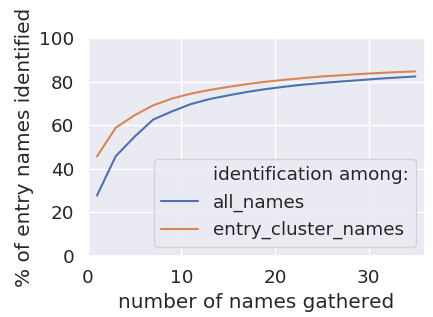
\includegraphics[width=.7\columnwidth]{images/stability_analytic.png}
	\caption{\% of objects for which the entry-level name can be confidently identified after gathering N names.}
	\label{fig:entry-level-name-stability}
\end{figure}
For each object we estimated, on the basis of its \mn response set, how many names should have been gathered for the entry-level name (as defined on the basis of 36 names) to be the majority name among them with 95\% probability.
The blue line shows that, even after gathering 10 names, the entry-level name is sufficiently likely to be the majority name for only 68\% of objects (i.e.,~for 32\% of objects, there's a greater than 5\% chance of getting a different majority name).
Gathering 20 names increases this to 78\%.
Our verification results let us see that most of the remaining indeterminacy occurs within the entry-level name's \cluster:
the red line is computed by taking only names from the \cluster of the entry-level name into account:
by discarding names for other objects, the entry-level name for the intended object can be confidently identified more easily---but not by much, since names for the wrong object tend not to compete for `most frequent' anyway.
%% SHORTENING %% (An analogous plot for the subset of all adequate names essentially coincided with the red line, reflecting that most adequate names were intended for the same object as the entry-level name.)

Note that both lines in Figure~\ref{fig:entry-level-name-stability} stay well below 100\%, reflecting that for 15\%-20\% of objects even gathering 36 names is not enough for the entry-level name to come out as majority (95\% probability): differences in frequencies between the contenders are simply too small.
That is, for 15\%-20\% of objects we aren't sure that the \emph{sample} entry-level name we derive from \mn---what we defined as the entry-level name---in fact corresponds to the \emph{population} entry-level name.
This is not expected to affect our model comparison, but in principle gathering even more annotations could help for these cases---although it is also possible that some instances do not have a single, clear entry-level name within a mixed population, or even for a given individual.


%%%%%% BY SAMPLING, FOR GEMMA:
% For each object that has an adequate entry-level name (adequacy $<.5$ according to our Verification results), we randomly sampled (including duplicates) a list of 36 names using the proportions in ManyNames as sampling probabilities, and computed the lowest number of collected names (i.e., the lowest index in the list) after which the entry-level name would reliably remain the most frequent one.
% We did this 30 times for each object.
% The blue line in the figure shows that, after collecting 10 names, the entry-level name is reliably identified for on average around 85\% of objects; collecting 20 names increases this to 90\%.\footnote{
%	But even when gathering 36 names, for around 6\% of objects this can still result in a different entry-level name. This reflects the existence of objects with no clear entry-level name, e.g., where two (almost) equally frequent names are both candidates.
%	\mw{Can we quantify this?}
%}
%The red line shows the same tendency but by taking only names from the entry-level cluster into account (as identified by our Verification results):
%by discarding names for other objects, the entry-level name for the intended object can be identified slightly more quickly (but not by much, since names for the wrong object tend to be a minority anyway).
%\begin{figure}[t]
%	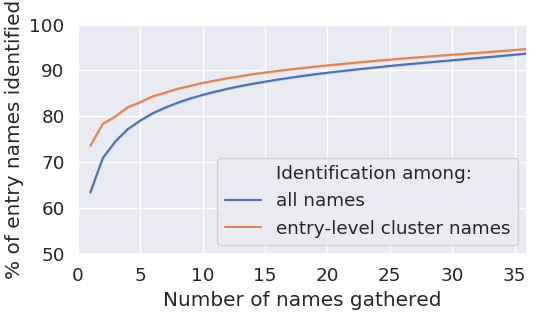
\includegraphics[width=\columnwidth]{images/stability-all-05-05-spellchecked.png}
%	\caption{}
%	\label{fig:entry-level-name-stability}
%\end{figure}


%%% mode: latex
%%% TeX-master: "acl2020_main"
%%% End:
